% !TEX encoding = IsoLatin2  % notwendige Zeile f"ur Mac-Benutzer (muss als Kommentar stehen); Windows-Benutzer k"onnen
%die Zeile l"oschen.

% LaTeX-Vorlage Version 3.1,  Juli 2011
% erstellt von Dr. Andreas Drauschke (andreas.drauschke@technikum-wien.at) und Dr. Susanne Teschl (susanne.teschl@technikum-wien.at)
% geringf"ugig adaptiert von Harald Stockinger (harald.stockinger@technikum-wien.at)


\documentclass[11pt,a4paper,bibtotoc,oneside]{scrbook}
% F"ur kurze Arbeiten w"are auch die Dokumentklasse "scrartcl" ausreichend. In diesem Fall ist "section" die h"ochste Ebene ("chapter" gibt es dann nicht).
% \documentclass[a4paper,bibtotoc,oneside]{scrartcl}


%Zum Verlinken des inhaltsverzeichniss & co
\usepackage[colorlinks=false]{hyperref}
% %hyperref setup`%
\hypersetup{pdfborder=0 0 0}
%       colorlinks=false,
%       citecolor=Violet,
% %         linkcolor=Green}
\usepackage[utf8x]{inputenc}
% deutsche Anpassungen
% \usepackage[ansinew]{inputenc}
\usepackage[T1]{fontenc}
\usepackage[ngerman]{babel}
% mathematische Symbole
\usepackage{amsmath,amssymb,amsfonts,amstext}
\usepackage{xcolor}
\usepackage{calc}
\usepackage{caption}
\usepackage{float}
%tabellen

% Kopfzeilen frei gestaltbar
\usepackage{fancyhdr}
\lfoot[\fancyplain{asdf}{}]{\fancyplain{}{}}
\rfoot[\fancyplain{}{}]{\fancyplain{}{}}
\cfoot[\fancyplain{}{\footnotesize\thepage}]{\fancyplain{}{\footnotesize\thepage}}
\lhead[\fancyplain{}{\footnotesize\nouppercase\leftmark}]{\fancyplain{}{}}
\chead{}
\rhead[\fancyplain{}{}]{\fancyplain{}{\footnotesize\nouppercase\sc\leftmark}}

% Farben im Dokument m"oglich
\usepackage{color}

% Schriftart Helvetica
\usepackage{helvet}
\renewcommand{\familydefault}{cmss}

% Graphiken einbinden: hier f"ur pdflatex
\usepackage[pdftex]{graphicx}
% Um pdf einzufügen
\usepackage{pdfpages}
\usepackage{array}

% H"ohe und Breite des Textk"orpers etwas gr"osser definieren
\setlength{\textheight}{260mm}
\setlength{\textwidth}{1.05\textwidth}

% weniger Warnungen wegen "uberf"ullter Boxen
\tolerance = 9999
\sloppy

% Anpassung einiger "Uberschriften
\renewcommand\figurename{Abbildung}
\renewcommand\tablename{Tabelle}

% %footers and headers
% % \usepackage{fancyhdr}
% % \pagestyle{fancy}
% \lhead{\studiumshort}
% \chead{}
% \rhead{\fachnameshort}
% \lfoot{\teilnehmeronenachname, \teilnehmertwonachname}
% % \cfoot{erstellt am: \today}
% \rfoot{\thepage}
% \renewcommand{\headrulewidth}{0.5pt}
% \renewcommand{\footrulewidth}{0.5pt}
\usepackage{geometry}
\begin{document}
% Kopf- und Fusszeilen initiieren
\pagestyle{fancy}

% Deckblatt:
\thispagestyle{empty}
\begin{picture}(0,0)
\color{white}\sffamily
\put(-101,-390){
\includegraphics[width=1.002\paperwidth]{./picture/LPS_2011.pdf}}
\put(220,-670){
\includegraphics[width=0.5\textwidth]{./picture/FHTW_Logo_4c.pdf}}
\put(-30, -20){\bfseries\huge PROJEKTARBEIT}
% Titel des Studienganges einf"ugen:
\put(-30,-50){\Large im Studiengang BEL4}
% Titel der Lehrveranstaltung einf"ugen:
\put(-30,-70){\Large Lehrveranstaltung Embedded Systems Software Design}
\color{black}
% Titel der Arbeit einf"ugen:
% Die Minipage wird gesetzt, damit auch mehrzeilige Titel m"oglich werden.
\put(-32,-350){
\begin{minipage}{13cm}
\bfseries\huge CNC-Machine
\end{minipage}
}
% Name der Autorin/des Autors eingeben:
\put(-30,-450){\large Ausgeführt von:\ Alexander Rössler }
\put(+54,-470){\large \ Johannes Wimmer}
\put(+204,-450){\large \ Koroosh Pirghaibi }
\put(+204,-470){\large \ }
\put(-30,-490){\large Matrikelnummer: 1110254020}
\put(+63,-510){\large 1110254023}
\put(+210,-490){\large 1110254003}
\put(+210,-510){\large }

\put(-30,-550){\large Begutachter: Dr. Martin Horauer}
\put(-30,-590){\large Wien, \today} % das Datum des letzten Kompilierens wird automatisch eingesetzt
\end{picture}
\savegeometry{GEO1}
\newpage

\tableofcontents\thispagestyle{empty}
\newpage

\setcounter{page}{1}
\newgeometry{top=25mm, left=30mm, right=30mm, bottom=25mm, headsep=2mm, footskip=13mm}
\savegeometry{GEO2}
% Falls die Kapitel"uberschriften zu lang f"ur die Kopfzeile oder das Inhaltsverzeichnis sind, so erzielt man
% dort Kurzformen der Kapitelbezeichnungen mittels:
% \chapter[Kurzform]{Lange "Uberschrift}
\chapter{Projektbeschreibung}

%=====================================================================================================================%
\section{Ziel}
Das Ziel dieses Projekts ist der Entwurf, Implementierung, und der Test einer Embedded Software mit der Hilfe von einem „eStick“  und einem „Embedded Artists LPCXpresso baseboard“ für eine CNC-Maschine. Die Maschine, welche im Rahmen dieses Projekts verwendet wurde, ist die Zentoolworks mit der Microschritt-Leistungsendstufe SMC11.

\section{Funktionsweise}
Über eine graphische Oberfläche werden Befehle und Koordinatendaten des abzuarbeitenden Musters über USB an einen LPC1758 gesendet. Der Microcontroller steuert die Treiberstuffen (SMC11G) der Schrittmotoren.\\\\
Die SMC11 ist eine kompakte Mikroschritt-Leistungsendstufe zur Ansteuerung von 4-, 6- und 8-Leiter-Schrittmotoren.  
Die SMC11 bietet folgende Funktionen: 

\begin{itemize}
\item Ansteuerung der Eingänge „Takt“, „Richtung“, „Enable“ und „Stromabsenkung“ 
über 3,5 V Low Voltage Prozessoren oder über ein 3,5 V bzw. 5 V TTL-Signal 
möglich. 
\item Automatische Stromabsenkung: um die thermische Belastung des 
Motors und der Endstufe im Stillstand zu reduzieren. Wird der Phasenstrom nach
einer Taktpause von maximal 1,5 sek. automatisch auf < 50 Prozent des  eingestellten Wertes abgesenkt. 
\end{itemize}
Bei der Implementierung wurden insgesamt 4 Tasks angelegt:
\begin{itemize}
\item Start-Task
\item Button-Task
\item Motorsteuerung-Task
\item USB-Connection-Task

\end{itemize}

\chapter{Umsetzung}

\section{Desktop Server}
\subsection{Funktionalität}
    \begin{figure}[H]
    \centering
        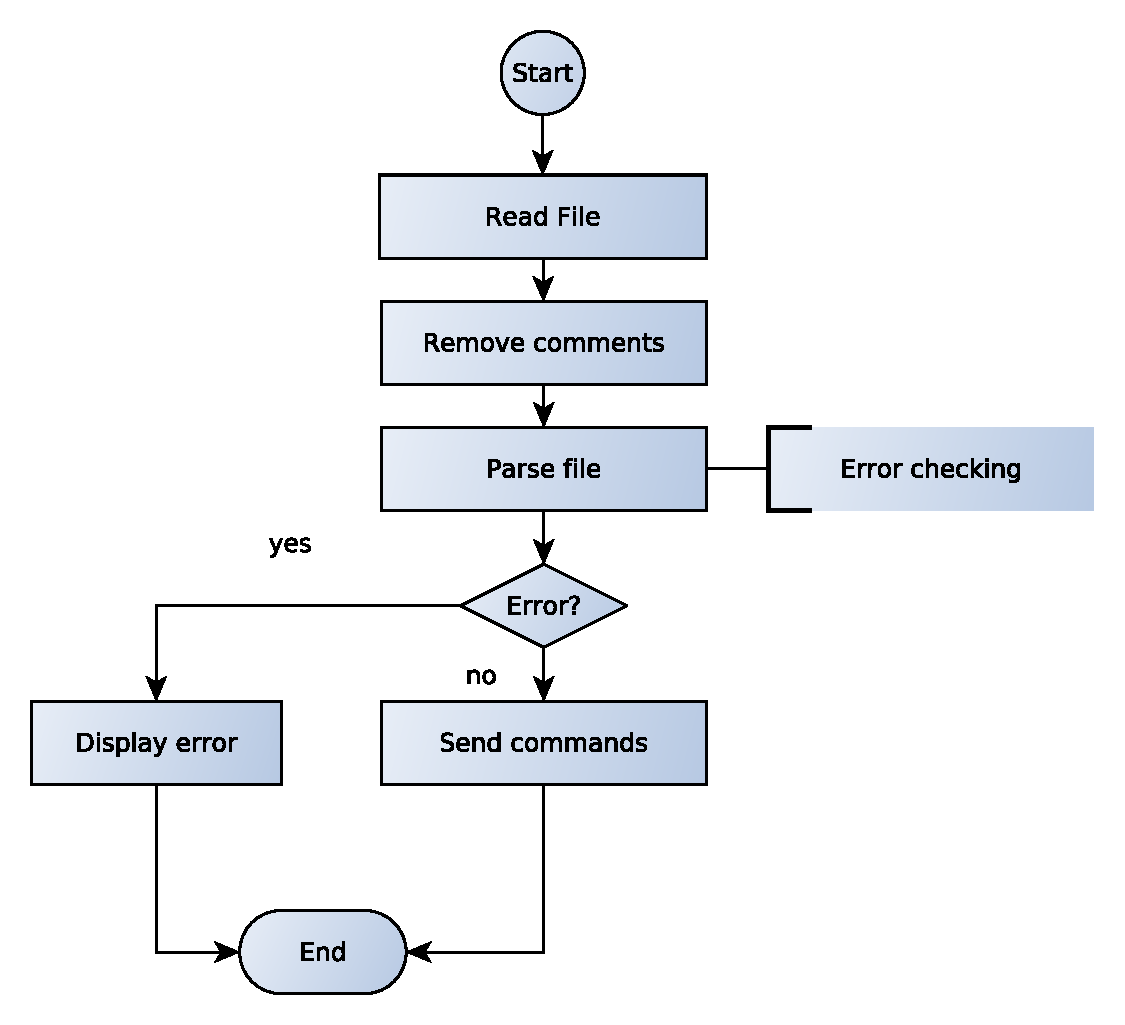
\includegraphics[width=200pt]{./picture/process1.pdf}
        \caption{\label{main}{Processing a GCode-file}}
    \end{figure}
    
        \begin{figure}[H]
    \centering
        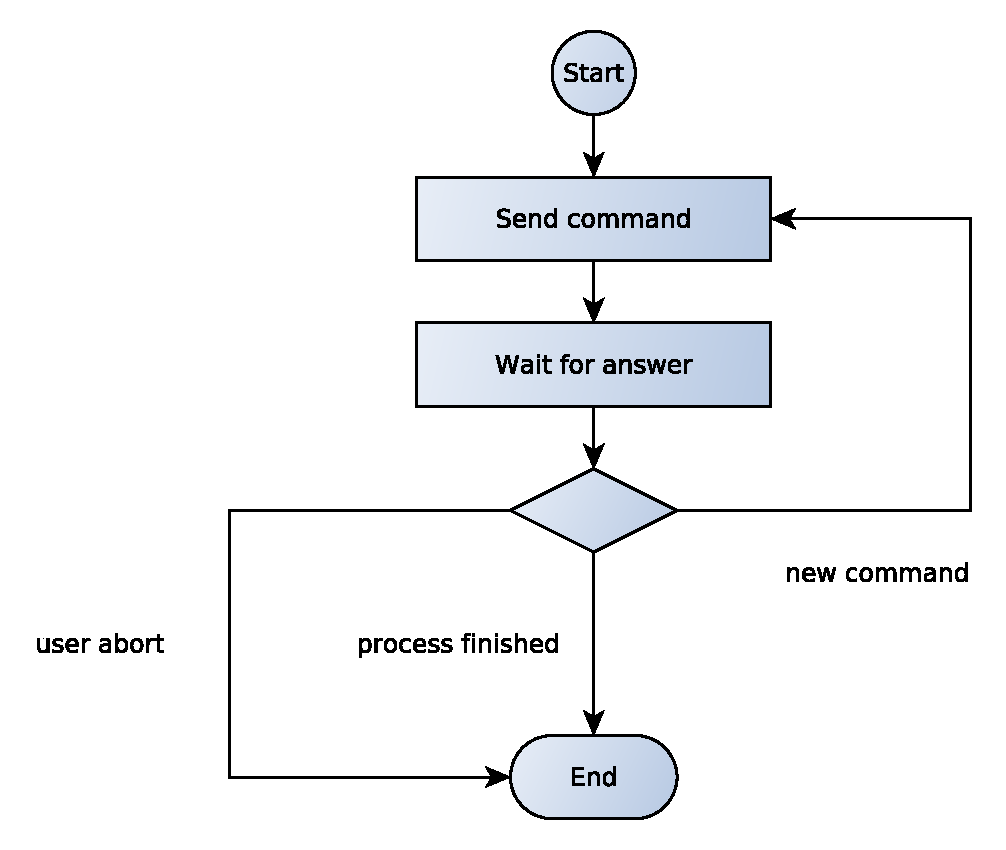
\includegraphics[width=200pt]{./picture/process2.pdf}
        \caption{\label{main}{Server-side communication}}
    \end{figure}

\subsection{GUI}
Die GUI wird in zwei Fenstern implementiert. Das Hauptfenster enthält alle Elemente um die Maschine anzusteuern und Ausgaben zu loggen.
Das Preview Window dient nur zur Visualisierung des Pfades.
\subsubsection{Mockup}
    \begin{figure}[H]
    \centering
        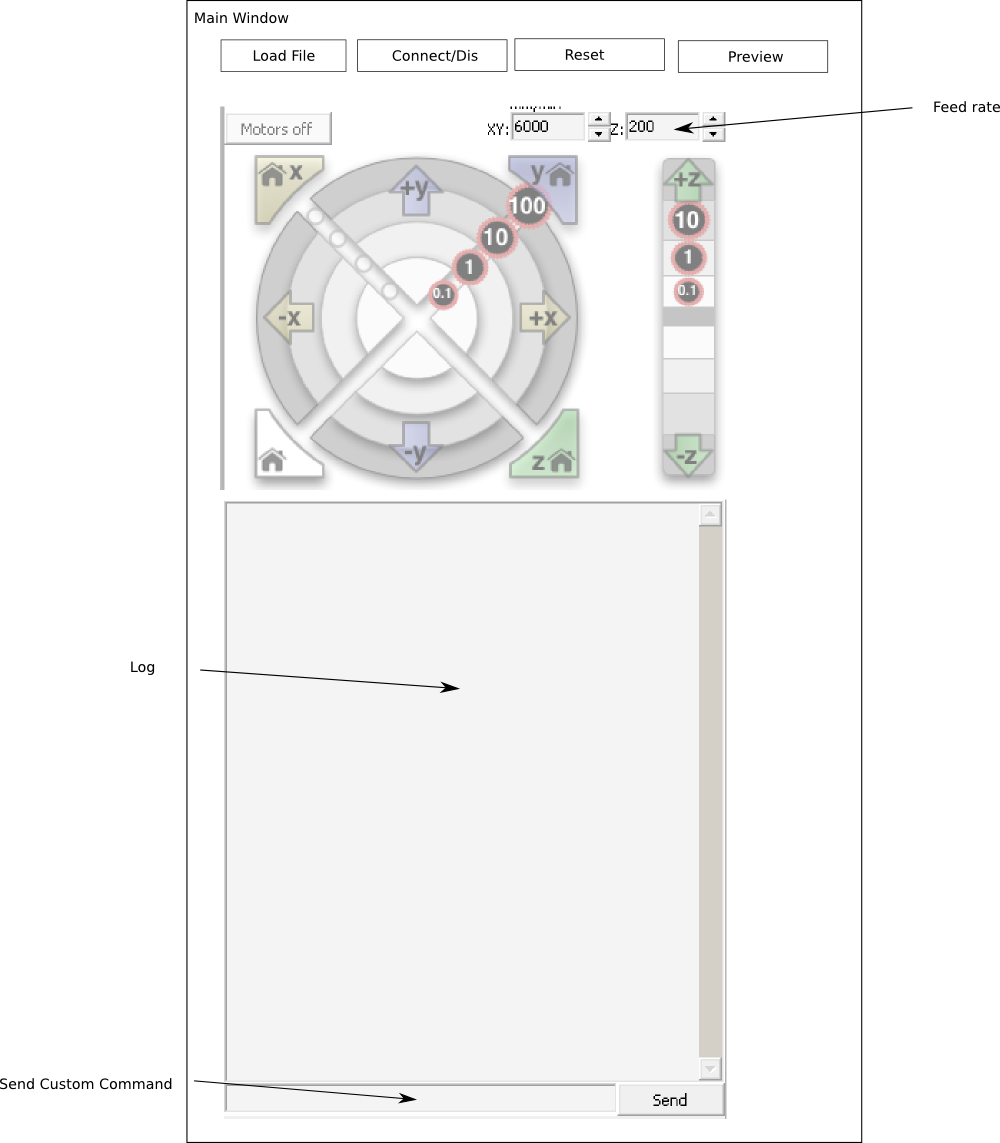
\includegraphics[width=260pt]{./picture/gui_main.png}
        \caption{\label{main}{Main Window}}
    \end{figure}
    
    \begin{figure}[H]
    \centering
        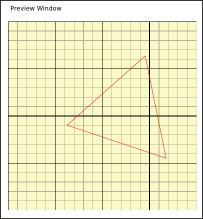
\includegraphics[width=200pt]{./picture/gui_preview.png}
        \caption{\label{main}{Preview Window}}
    \end{figure}

\chapter{Kommunikation}
\begin{figure}[!ht]
    \centering
        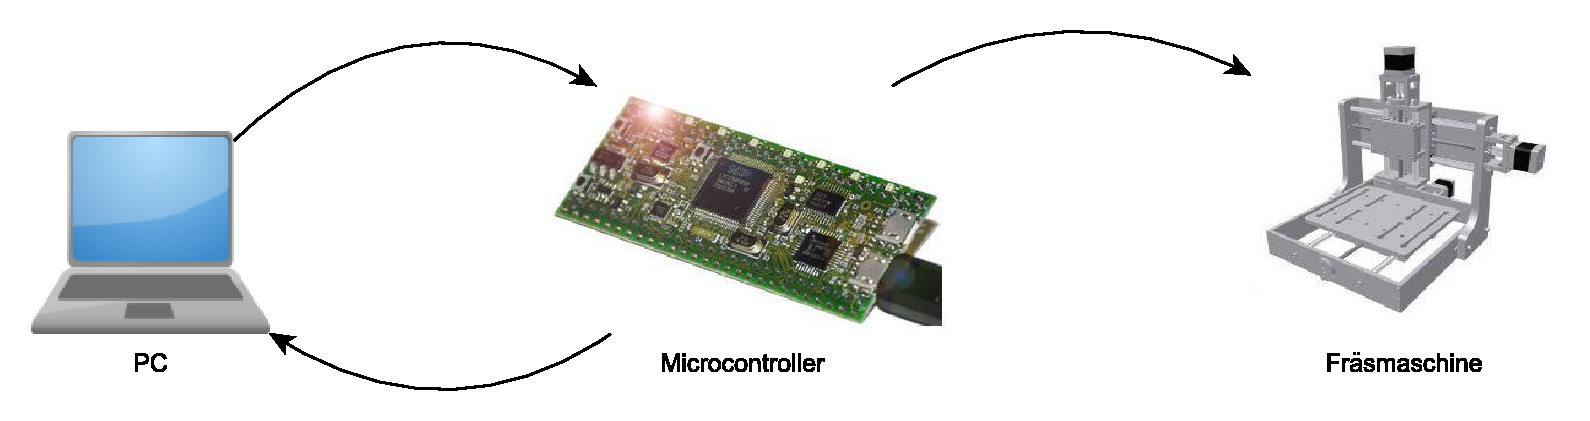
\includegraphics[width=360pt]{./picture/Kommunikation.pdf}
        \caption{\label{lm324}{Kommunikation}}
\end{figure}
\section{Kommunikation zwischen dem PC und dem Microcontroller}
Die Kommunikation zwischen dem PC (GUI-Aplikation) und dem Microcontroller erfolgt über USB. Drei G-Code Befehle werden jeweils von der graphischen Oberfläche an den Microcontroller geschickt. Nach dem Abarbeiten der ersten drei Befehle werden drei neue Befehle an den Microcontroller geschickt. Der Microcontroller liefert einen Finish-Befehl an die graphische Oberfläche, wenn er am Ende von dem G-Code angekommen ist.\\\\
Das Steuerkreuz sendet je nach Button 0.1, 1, 10 oder 100 mm Schritte an den Microcontroller.
\section{Kommunikation zwischen dem Microcontroller und der Motorsteuerung}
Wenn der USB-Empfangspuffer nicht leer ist, wird der empfangene Befehl in Einzelbefehle, die durch Leerzeichen getrennt sind, aufgesplaten. Die Koordinatenwerte und die Geschwindigkeitswerte der einzelnen Befehle werden in einem Puffer gespeichert. Der regelmäßig aufgerufene Task Motorsteuerung ruft während des Zustands „working“ eine Funktion auf, die je nach eingestellter Geschwindigkeit auf allen Achsen eine gewisse Anzahl an Schritten abfaehrt. \\
\\Andere Befehle wie homing, calibration, oder Abbruch werden direkt nach dem Empfang von USB-Task aufgerufen.

\section{Kommunikation zwischen der Motorsteuerung und der Fraesmaschine}
Die von der Motorsteuerung aufgerufene Funktion holt die aktuellen Werte aus dem Puffer, startet den Timer, und setzt die Richtung. Beim Ablauf des Timers wird jedes Mal die Taktflanke für den Schrittmotor getoggelt. Nach dem die Schritte, welche zu fahren sind, abgearbeitet sind, wird der Timer und somit der Motor gestoppt.

 %\begin{figure}[!ht]
 %   \centeringe
 %       \includegraphics[width=260pt]{./picture/LM324_triangle.png}
        % LM324_triangle.png: 0x0 pixel, 250dpi, 0.00x0.00 cm, bb=
 %       \caption{\label{lm324}{Ausgangssignal LM324}}
 %   \end{figure}

%\restoregeometry

%\bibliographystyle{IEEEtran}
%\bibliography{Literatur}

% Abbildungsverzeichnis
% \listoffigures
% \addcontentsline{toc}{chapter}{Abbildungsverzeichnis} % f"ugt den Eintrag "Abbildungsverzeichnis" im Inhaltsverzeichnis hinzu
% % \newpage
%
% % Tabellenverzeichnis
% \listoftables
% \addcontentsline{toc}{chapter}{Tabellenverzeichnis} % f"ugt den Eintrag "Tabellenverzeichnis" im Inhaltsverzeichnis hinzu
% % \newpage

% Abk"urzungsverzeichnis
% Bei Verwendung der Dokumentklasse "scrartcl" ist der Befehlt \addchap{Abk"urzungsverzeichnis} durch
% \addsec{Abk"urzungsverzeichnis} zu ersetzen
\addchap{Abk"urzungsverzeichnis}
\hspace{-17mm}\begin{tabular}{>{\raggedleft}p{0.2\linewidth} p{0.75\linewidth} p{0.1\linewidth}}
CNC  & Computerized Numercial Control \\
GUI  & Graphical User Interface \\
USB  & Universal Serial Bus \\

\end{tabular}

% Anh"ange
% \begin{appendix}
% \chapter[Erster Anhang]{Entwicklung und Aufbau eines Klasse D-Verstärkers}
% % \lhead{}
% % \lhead{\textcolor{blue}{\url{www.widatec.com/}}}\label{Anhang1}
% % \includepdf[pages={1-24},addtotoc={{24},{section},{2},{Entwicklung und Aufbau eines Klasse
% % D-Verstärkers},{D-Verstärker}}, pagecommand={\thispagestyle{fancy}},noautoscale=true,width=1.1\textwidth,offset=0cm
% % 1cm]{/home/christian/FH/3.Semester/ATK/Projekt/seminararbeit1/unterlagen/CAE.pdf}
% % \lhead{\studiumshort}
% %
%
% \chapter[Zweiter Anhang]{"Uberschrift des zweiten Anhangs}
%
% Text Text Text Text Text Text Text Text Text Text Text Text Text Text Text Text Text Text Text Text Text Text Text Text ...
%
% \end{appendix}

\end{document}
